\section{Design} 

\subsection{Server Architecture}

Realizing the academic goals of this work, each of the server components has been separated in well differenced and independant modules. This is to minimize coupling and maximize cohesion. Each module follows a defined interface. By making use of interfaces, methods do not know how the modules are implemented.
This allows modifying a module�s implementation without affecting the ones who access it, as long as the shown interfaces are still complied.

This approach is based on an object-oriented design, using different design patterns to ease the understanding of each module and to provide standard solutions. Every object has a specific purpose, which allows to a better comprehension of each module�s code and the engine�s inner work.

Figure 1 shows existing relationships between modules. When a Client establishes a connection to the Server, the Listener component accepts it and asks the Thread Factory module for the creation of a thread, so the Executor can use it to provide a response to the connection request. Then, the Executor component communicates with the different modules involved in the answering of the query. In addition, the figure shows the relationship between the Client and the Back Listener component. This one is in charge of gather together action produced in the Lock Manager and every record written in the Log file, so they can be visualized in a user-friendly way.

\begin{figure}[ht]
		\centering
		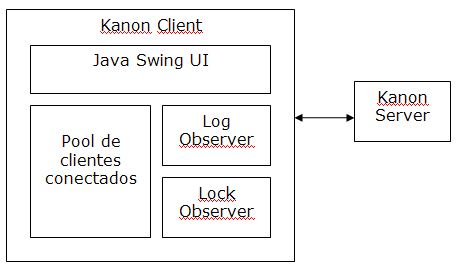
\includegraphics[scale=0.5]{img/arquitectura.png}
		\label{fig:arquitectura.png}
		\caption{Kanon Server Architecture}
\end{figure}

The following sections explain with detail those components that have a greater relevance with the aim of this work. Emphasis on the ARIES family of algorithms is shown where applicable, specially in the Recovery Manager section.


\subsection{Buffer Manager}

To handle frames and pages in the Buffer Manager, a \textbf{steal / no-force} approach is used. As \textbf{no-force} does not require the page to be saved on stable storage for every commit, that action can be taken when the last transaction that was modifying the page finishes, considerably reducing I/O actions. This enhancement combines with the \textbf{steal} approach, which allows a �still being modified� page to be saved on disk and erased from memory (to make room for a new one), increasing the engine�s virtual memory capacity. Later, if those changes have to be undone, the ARIES rollback algorithm executes, reading the log file to undo every operation performed on the pages.

ARIES also treats about the page access control. Buffer Manager pages can be locked in three different ways:

\textbf{pin}:
When a page is pinned, the removal algorithm of the Buffer Manager will not erase it from memory. A pinned page means that one or more active transactions are reading or writing on it. In this work, the Pin Manager sub module controls these operations. There is a counter to know how many transactions are accessing each page. The Pin Manager increments a page counter by one when a transaction needs the associated page, and decrements it by one when the transaction releases that page.

\textbf{latch}:
If several transactions concurrently try to update a page, they have to do it in order. Therefore, every time they do it they try to acquire a latch on the page and if they cannot, they enqueue the request and wait for the latch to be released. Each page has a variable that points to the last ARIES update log event that was realized on the page. For reading operations, no latch is needed.
There is a Latch Manager sub module that controls all these operations.

\textbf{lock}:
The Lock Manager component is in charge of page locking. A transaction could use it if it has locked several records from a page (optimization purposes). This work does not use page locking in any way.

\subsubsection{Deadlock prevention between latches and locks}
 
ARIES documentation shows the steps to follow to avoid a deadlock between record locks and page latches (also applies to indexes pages):

\textbf{update / delete}:
First, a transaction acquires an exclusive lock on the record, and then it obtains a latch on the page. If some other transaction already was in possession of that latch, because of how the algorithm works, it will not request a lock for any of already-locked record before releasing the latch.

\textbf{insert}:
First, a transaction attains a page latch, and then it asks for a new record ID. Then, It proceeds to \textbf{conditionally} lock that ID in an exclusively way, to insert the new record. If the conditional lock fails, it releases the latch and tries to \textbf{unconditionally} lock the ID. Once the lock is held, it requests a new page latch and verifies that the ID is still free. If it is not, the transaction releases the lock and then repeats the entire process.

The Buffer Manager has methods to get, release, create or delete a page; to know if some page is loaded in memory and to save to stable storage those pages that were modified. The Disk Space Manager is the one in charge for the persisting processes.

\subsection{Executor}
The Executor component, first calls the Analyzer to decompose the SQL query into understandable segments. Then, it solves the query and returns a response back to the Client.

Available isolation levels are Read Uncommitted, Read Committed, Repeatable Read, and Serializable. More information about isolation levels come out in the Lock Manager section.

\subsection{Recovery Manager}

The Recovery Manager module provides robustness to a database engine. It main functionality is to give Atomicity and Durability properties to the engine�s transactions \cite{RaGh03}.

Along the different techniques available to achieve this purpose, the most known ones are Shadow Paging (\cite{WISHAP}, \cite{RaGh03}), and Write Ahead Logging (\cite{WIWALO}, \cite{RaGh03}). One of the objectives of this work is to show the functionality of an ARIES based recovery system \cite{MHLPS89}, \cite{Moha99}. The ARIES family of algorithms uses a WAL strategy, as it is less expensive in memory use.

Each operation in the database is saved into a Log, specifying what kind of event is. It is also stored any parameters that the operation uses, so that it can be undone or redone if it is necessary. The Log file is in an increasing format, and must be saved in a persistent medium anytime a transaction commits, or when the engine performs a database checkpoint \cite{RaGh03}.

\begin{figure}[ht]
		\centering
		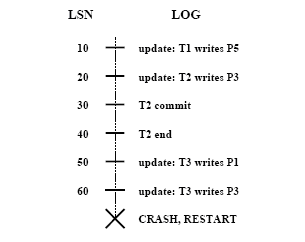
\includegraphics[scale=0.6]{img/LogHistory.png}
		\label{fig:LogHistory.png}
		\caption{Example of a Log History}
\end{figure}

When a transaction modifies a table page or an index page, ARIES standard recommends saving an event stating what page was modified and what bytes were changed inside it. Because of the academic goals of this project, this modification event is split into more logical events (insert, update or delete of a record). This allows to a better knowledge of the engine�s inner working, as that detailed operation will be in the Log. Therefore, a inspecting it will show up what type of modification was performed, which records it changed, and the before-and-after values.

Following ARIES proposal, each event has an identifier, based on its position inside the Log file. A transaction knows the ID of the last operation it executed, and every page in the database is aware of the ID of the last operation that was performed on it. When a transaction commits, it saves a commit event into the Log; and when a transaction ends, it stores an end event into the Log. When the engine decides to rollback a transaction, every associated event is undone from the last one to the first one. For every undo, a CLR-event is stored. A CLR-event is useful if the rollback has to be redone (for instance, there was a crash during the original rollback).

After a system failure, it is crucial that those modifications that were not stored persistently be redone, so the changes do not lost. It is also required that for those transactions actively executing during the failure and have not committed, to undo their changes, as if they never happened. ARIES conveys that the recovery steps that happen when the engine restarts, are divided in three phases �analysis�, �undo� and �redo�, and what to follow in each step. However, the procedural implementation proposed was altered for a more object-oriented approach.

To ensure that any modifications made by transactions be in a persistent storage, there exists the concept of a Checkpoint. A checkpoint forces the Log file into a persistent state, as well as persistence of any pages being held in the Buffer Manager memory. Regular database engines do a checkpoint in a periodic fashion, but this one does not do that so the Recovery system can be seen working when a failure occurs. Nevertheless, there is the possibility to force a checkpoint manually through a SQL query, and to force a system crash as well.

The recovery module and log subsystem support nested transactions, following the algorithms depicted in ARIES/NT \cite{RoMo89}.

In addition, there are some events inside a transaction that should not be undone, even if the transaction is rolled back. To achieve this functionality, Nested Top Actions were implemented \cite{MHLPS89}.

\subsection{Transaction Manager}

The purpose of this component is to manage the execution of all currently active transactions. Its structure holds every transaction running on the Server. For every connection established, there may be a transaction running for it (or several nested transactions). A transaction belongs to a thread. It cannot be suspended and resumed in another one.

There are some queries which should be executed inside a transaction, and other one for which a transaction is not needed. For instance, DML instructions must run within an active transaction, but the checkpoint query does not need to. As a result, if a query needs to be run within a transaction and there is no one actively running, the engine automatically creates one, runs the query, and commits it (or rolls back in case of failure). This decision means that each instruction that works on a data set runs entirely or does not run at all.

It is possible to create explicit transactions throughout SQL queries, like �Begin Transaction�, followed by the updating queries, and ended with a �Commit� or �Rollback�.

Every transaction has an ID number, which is atomically incremented every time a new transaction is created. Furthermore, at system start, the Log file is scanned to know the number of the last transaction executed so that a new transaction will start with a higher number and will not conflict with existing transactions stored in the log file.

Standard ACID properties are obtained in the following way:

\begin{itemize}
	\item Atomicity: When there is an error or a desire to rollback the transaction, ARIES-based Recovery Manager, using the Log file, does the rollback and undoes every modification made in each transaction operation to return the state of the database to the original state right before the beginning of the transaction.

	\item Consistency: As it is mentioned in \cite{RaGh03} section 18.1.1, end users are responsible to maintain consistency in held databases. This engine does not support integrity constraints, as primary keys, unique columns, or foreign keys.

	\item Isolation: Lock Manager guarantees serialization for those transactions concurrently executing. It additionally ensures locking for those transactions that wishes to access or update objects (records).

	\item Durability: As with atomicity, Recovery Manager takes into account the recovery of transactions that were active during a system crash. Every action that belonged to a committed transaction and was not saved in persistent storage is redone and then persisted. 
\end{itemize}

The Lock Manager section talks about transaction interleaving, scheduling, and isolation levels.

To give a deeper view into transaction processing, two ARIES extension were added into this engine, without giving away the educational goals of this work:
 
\subsubsection{Nested Transactions}
\cite{RoMo89} comments about adding nested transaction support to an ARIES-based recovery system. Marks log and event changes as well as modifications in the transaction table. Nested transactions were added to this work so people can look into advanced transaction functionality. One change is that for each thread, there is no more a pointer to the current active transaction, but a pointer to a list of transactions. That list is ordered in a sense that the top level transactions is first and the most recent and deepest one is at the bottom. 

When a nested transaction is created, it inherits the isolation level of its parent.

The rollback method of the Transaction Manager was replaced by two methods. The first one rolls back the most nested transaction of the thread, giving focus on its parent. The second one rolls back every transaction actively running in the connection, from the deepest one to the top-level one, leaving the connection in a state of no transaction running.

The commit method for a nested transaction writes an event that links it with its parent, so if the parent rolls back, every change made by it and by every nested transaction it had during its lifetime, is undone. The parent transaction updates its last LSN indicator to point to that nested commit event. 

Lock Manager and Recovery Manager Sections talk about changes made to each of them to support nested transactions.

\begin{figure}[ht]
		\centering
		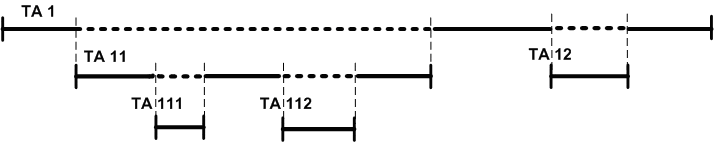
\includegraphics[scale=0.4]{img/TrxAnidadas.png}
		\label{fig:TrxAnidadas.png}
		\caption{Nested Transactions according to executing time}
\end{figure}

It is worth observing that when a nested transaction is created, the parent one is suspended, because each new query of the connection will belong to the new child transaction until it rolls back or commits. Therefore, it is not required to hide those changes made by the child to its parent, because it is suspended, and any transaction cannot have more than one child at any moment in time.


\begin{figure}[ht]
		\centering
		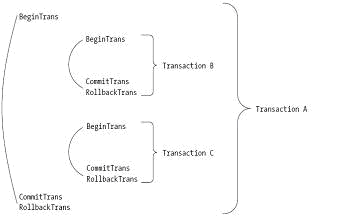
\includegraphics[scale=0.7]{img/TrxOperaciones.png}
		\label{fig:TrxOperaciones.png}
		\caption{Nested Transactions as operations}
\end{figure}

\subsubsection{Savepoints}

A savepoint permits establishing a significant point inside an active transaction, and allows undoing any modifications made since that point and forward. Use of these savepoints is exposed to the user interface as SQL queries for their creation and use (transaction rollback up to the savepoint).

To the end user, each savepoint has a friendly name. Then those names are associated with the last LSN (log event, see Recovery Manager Section) of the active transaction. If a savepoint existed with the same name, it is deleted. On the other hand, there can be savepoints with the same name across different active transactions. This statement includes nested transactions, as it is not possible to roll back to a savepoint that belongs to some parent transaction.

\begin{figure}[ht]
		\centering
		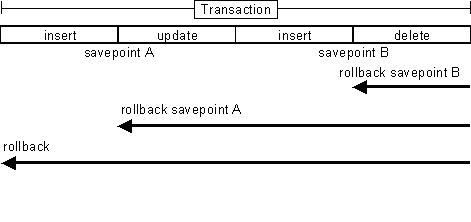
\includegraphics[scale=0.6]{img/trxSavePoints.png}
		\label{fig:trxSavePoints.png}
		\caption{Use of savepoints}
\end{figure}

Taking advantage of this savepoint support, when queries are performed inside an explicitly active transaction a savepoint is automatically marked before each execution, thus if an exception occurs, the transaction rolls back to that mark. This assertion excludes dead lock exceptions, as in that case all the transactions that belonged to the victim thread are rolled back, to release any lock they could have held.

\subsection{Index Manager}

This module was built to enhance transaction performance during concurrent queries. It provides a simple hash index for every table stored in the catalog. As table records are stored unordered, these indexes are known as \textit{unclustered}. And as there is an entry for each record within the table, they are also \textit{dense}. It should be mentioned again that this engine does not implement primary keys or unique constraints on table columns, so the Index Manager provides secondary indexes. In section 8.4 of \cite{RaGh03} it is explained all kind of index properties available.

The main objective of this component is that for every query where an index can be used, to use it instead of run a full table scan. In higher isolation levels, a full scan would lock all the table records, diminishing concurrency if other transaction wants to modify a record at the same time. With indexes, only those records that match the \textit{where} clause will be locked for reading. An index is useful for \textit{serializable} isolation as well, because without them, the entire table would have to be locked to prevent the insertion of a new record that would result in the same query to return a different answer inside the same transaction.

Indexes are stored in buckets with overflow (Hash indexes with overflow are explained in chapter 10 of \cite{RaGh03}). Every possible value of a column is assigned to a hash number, and a bucket entry that has the structure [column, hash number] is added. As this is not a dynamic index, some hash entry may have many more buckets in comparison with some other entry, but it still will yield in a more concurrent execution than to run a full table scan. 

These hash indexes are also useful to avoid fully scanning the system tables. For instance, when a table must be retrieved, only those records that point to a table which name has the same hashing number than the name of the required table are searched.

The ARIES family of algorithms permits that the pages that hold the index buckets are as transactional and recoverable as normal table pages. Logic events where added to the log that represent an index update or removal, with the corresponding UNDO and REDO operations, if they are needed. Index locking was added to the Lock Manager for isolation purposes (more details in the Lock Manager Section). Latches are used when some bucket is modified, in the same manner than pages.

\subsection{Lock Manager}

It manages reading and writing locks. A pessimistic lock is used  \cite{RaGh03} because it is simpler than the version control usually used in optimistic locking.

The Two phase locking protocol was implemented, over the RLOCK / WLOCK scheme (ternary locks). First it was thought following that is written in chapters 18 and 19 of \cite{RaGh03}. It supports record-granularity locking, allowing greater concurrency between transactions.

\begin{figure}[ht]
		\centering
		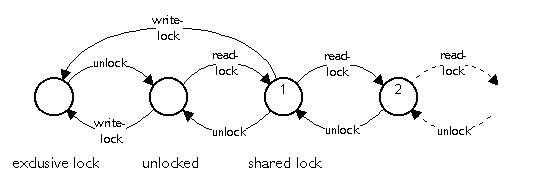
\includegraphics[scale=0.6]{img/LockManager.png}
		\label{fig:LockManager.png}
		\caption{Two-phase-locking model}
\end{figure}

The four standard isolation levels have been implemented: \textbf{read uncommitted}, \textbf{read committed}, \textbf{repeatable read} and \textbf{serializable} \cite{WIISLE}, \cite{RaGh03}. Element locking inside a transaction holds to strict 2PL protocol for the first two levels \cite{WIS2PL}, and rigorous 2PL for the latter two \cite{WIR2PL}. As it is shown in \cite{BGLL99} and \cite{Fran92}, semantic correctness holds and the different levels show a tradeoff between performance (less blocking / greater concurrency) and possible inconsistencies in transaction's isolations.

Lock Manager was designed as follows: 

There are methods to lock an object (using the object's ID), to unlock it, and to know if an object is locked.

When locking an object, it has to be specified if it is going to be an exclusive lock or a shared one. In this scheme, exclusive locking is used before modifying the object, and shared locking for object to be accessed without any modification. These methods are executed in a synchronized way. That means that only one transaction at a time may be executing them. This was a requirement because locking structures and tables are shared between different connections.

Just as other modules that are related to transaction processing, this manager was later modified to add support for nested transactions and savepoints.

When a transaction rolls back up to a Savepoint, every lock that was acquired after that savepoint is released. To accomplish that, it is known what the last LSN in the transaction right was before obtaining the lock.

When a nested transaction is created, it inherits every lock possessed by its parent. Each lock knows which transaction created it. To know if an object is already blocked by some transaction, the algorithm has to check not only those objects locked by it, but also those that were locked by any transaction ancestor. When a child transaction is aborted, every lock that was created inside it is released. But when a child transaction commits, the locks that it owned are not released, but transferred to the parent transaction. This process repeats for every child transaction that is committed until the top level transaction is reached.

A special case occurs when a parent transaction holds a shared lock to an object, and the child transaction wishes to upgrade that lock to an exclusive one (to later modify the object). If that happens, both locks are recorded in the locking structures, so when the child transaction ends, the exclusive lock is passed to the parent, effectively upgrading the shared lock it possessed.

\subsubsection{Deadlocks}

For deadlock treatment, it was decided to rely on deadlock prevention algorithms instead of deadlock detection ones. This is to mantain simplicity in the project. As as future work, the latter ones could be implemented. An interface was designed, which is used by the Lock Manager every time an object is going to be locked, to verify if there may be some kind of conflict between the transaction that wishes to lock and those ones that already own some lock on the desired object.

\subsection{Architechture and design of Kanon Client}

\begin{figure}[ht]
		\centering
		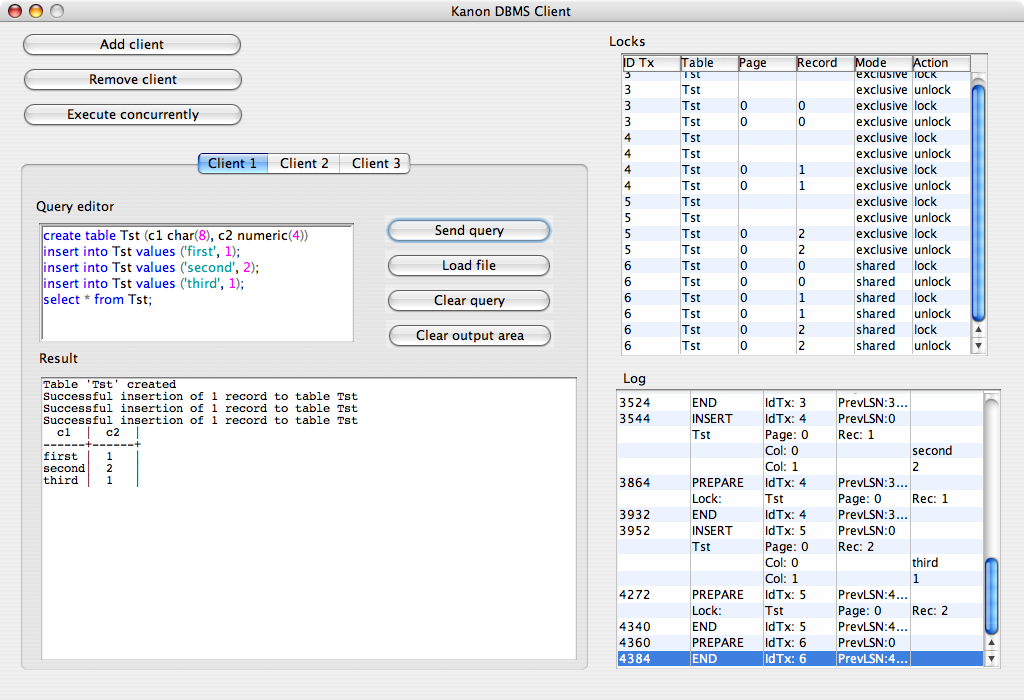
\includegraphics[scale=0.33]{img/KanonClienteMac.png}
		\label{fig:KanonClienteMac.png}
		\caption{Screen capture of a working Kanon Client }
\end{figure}

A visual client was built to test and verify the correct working of the engine.

These are its main characteristics:
\begin{enumerate}

\item In the main area, there are buttons to add and remove Client connections to the Server. For each new client connection, a new panel appears in the Tab Section. There is a button to send individual client queries to the Server. In addition, all the written queries of the different connected clients can be sent at the same time, to test transaction concurrency.

\item The tab area contains a panel for each connected client, and has buttons to handle the queries to the Server: 

\begin{itemize}

	\item Send the query written by the user in the query editor to the Server.
	
	\item Load a query from a file to the query editor.
	
	\item Clear the query editor.
	
	\item Clear the responses console.
		
\end{itemize}

\item The Lock panel is updated in real time. This permits observing transaction behavior as each query is being processed in the engine. Each lock entry specifies which kind of locking (or unlocking) was performed, and which object was locked. So it can be seen the restrictions of the two-phase-locking protocol, the concurrency of those transactions that access the same object at the same time, and the order they do that according to the selected isolation level.

\item The Log panel shows all the events that are being recorded to the log for each active transaction, and what ARIES does when a rollback occurs, what it does when nested transactions are used, and what happens during the recovery process (in each of the three steps defined by ARIES).

\end{enumerate}
